\documentclass[laboratorio]{guia}

\def \practnum {5} 
\def \practica {Circuitos RC y RLC}

\def \materia {Laboratorio de F\'\i sica II para Qu\'\i micos}
\def \periodo {2do. Cuatrimestre de 2015}
\def \catedra {Pablo Cobelli}
\def \website {http://materias.df.uba.ar/f2qa2015c2}
 
\usepackage{graphics}
\usepackage{amsmath}
\usepackage{amsfonts}
\usepackage{graphicx}
\usepackage{float}
\usepackage{wrapfig}
\usepackage{subfigure}
\usepackage{bm}
\usepackage{grffile}
\usepackage{color}
\usepackage{framed}
\usepackage[utf8]{inputenc}
\usepackage[T1]{fontenc}
\usepackage{lmodern}
\usepackage{circuitikz}
\usepackage[spanish]{babel}
\usepackage{babelbib}
\selectbiblanguage{spanish}

 

%----------------------------------------------------------
% Agrega al path de figuras el subdirectorio con el mismo
%     nombre que el archivo principal del proyecto
\graphicspath{{./\jobname/}}

%----------------------------------------------------------
% Definicion del entorno 'sabermas'
\makeatletter
\definecolor{shadecolor}{rgb}{0.89,0.91,0.94}
\newenvironment{sabermas}[1]{%
\vfill
\begin{shaded}
  \begin{center}
  {\textsection{Para saber m\'as}}
  \end{center}
  #1
\sf } 
{%
\end{shaded}%
}
\makeatother

%----------------------------------------------------------
% Definicion del entorno 'problema'
\newcounter{ContadorProblema}
\setcounter{ContadorProblema}{0}
\newcounter{TieneFiguraAsociada}
\setcounter{TieneFiguraAsociada}{0}
\newcounter{UbicacionFigura}
\setcounter{UbicacionFigura}{0}

\newenvironment{problema}[2][]
{%
    \ifx\relax#1\relax%
        \setcounter{TieneFiguraAsociada}{0}
        \else
        \setcounter{TieneFiguraAsociada}{1}
    \fi
    \def \archivofigura {#1}
    % 
    \refstepcounter{ContadorProblema}
    \noindent%
    \ifnum\value{TieneFiguraAsociada} < 1%
        {\sffamily \bfseries Problema \arabic{ContadorProblema}.}
        %{\sc {#1}}%
        \par\nobreak\par\nobreak%
        \medskip 
    \else
        % Va con figura; resta determinar de que lado.
        \ifnum\value{UbicacionFigura} < 1
            % Poner la figura del lado derecho
            \begin{minipage}{12.25cm}
            {\sffamily \bfseries Problema \arabic{ContadorProblema}.}
            %{\sc {#1}}%
            \par\nobreak\par\nobreak%
            \medskip 
        \else
            % Poner la figura del lado izquierdo
            \begin{minipage}{4.5cm}
                \centering
                \includegraphics[width=4.5cm]{\archivofigura}
                {\footnotesize {\sffamily Esquema asociado al 
                problema \arabic{ContadorProblema}}.}
            \end{minipage}\hfill%
            \begin{minipage}{12.25cm}
                {\sffamily \bfseries Problema \arabic{ContadorProblema}.}
                %{\sc {#1}}%
                \par\nobreak\par\nobreak%
                \medskip 
        \fi
    \fi
}
{%
    \ifnum\value{TieneFiguraAsociada} < 1%
        % \par \bigskip \vskip 0.3cm
    \else
        % Va con figura; resta determinar de que lado.
        \ifnum\value{UbicacionFigura} < 1
            % Poner la figura del lado derecho
            \end{minipage}\hfill%
            \begin{minipage}{4.5cm}
                \centering
                \includegraphics[width=4.5cm]{\archivofigura}
                {\footnotesize {\sffamily Esquema asociado al 
                problema \arabic{ContadorProblema}}.}
            \end{minipage}
        \else
            % Poner la figura del lado izquierdo
            \end{minipage}%
        \fi
    \fi
    \setcounter{TieneFiguraAsociada}{0}
    \par \bigskip \vskip 0.3cm
    % Permutamos el valor de la ubicacion
    \ifnum\value{UbicacionFigura} < 1
        \setcounter{UbicacionFigura}{1}
    \else
        \setcounter{UbicacionFigura}{0}
    \fi
}

%----------------------------------------------------------
% Definicion/Redefinicion de estilos
\renewcommand{\vec}[1]{\ensuremath{\mathbf{#1}}}



\hyphenation{ coe-fi-cien-tes coe-fi-cien-te au-to-va-lor
              au-to-va-lo-res co-rres-pon-der pro-ble-ma 
              cual-quie-ra po-la-ri-za-cio-nes }

\graphicspath{{./Guia_05_Circuito_RC/},{./Guia_06_Circuito_RLC/}}

\begin{document} 
\objetivo{{\bf Circuito RC:} Estudiar el r\'egimen transitorio de un circuito RC, tanto en la 
    etapa de carga como de descarga del capacitor, determinando experimentalmente
    los tiempos caracter\'\i sticos de evoluci\'on. 
    {\bf Circuito RLC:} Determinar experimentalmente la frecuencia de resonancia en un circuito
RLC serie. Medir el desfasaje entre la tensi\'on y la 
corriente en funci\'on de la frecuencia de operaci\'on del circuito.   
    \tematicas{Circuitos de corrientes variables en el tiempo, RC, carga y
        descarga de un capacitor, tiempo caracter\'\i stico, circuito RLC serie, resonancia.}} 
\maketitle

\section{Circuito RC}

\subsection{Introducci\'on}

Considere el circuito RC mostrado en la Figura \ref{fig:circuitoRC}, en el
cual el capacitor se encuentra completamente descargado inicialmente y la
llave S, abierta. Al cerrarse esta \'ultima, la diferencia de potencial
$V$ impuesta por la fuente genera una corriente $I$ en el circuito. Esta 
corriente tendr\'a el efecto de llevar cargas de signo opuesto a las caras 
del capacitor. Resulta intuitivo que esta corriente no ser\'a constante en el tiempo; 
en particular esperamos que la misma se anule cuando el capacitor se haya
cargado. 


Un capacitor de capacidad $C$ conectado a una fuente de tensi\'on $V$ constante 
adquiere una carga $q = C V$. Esto nos permite conocer la ca\'\i da de
potencial sobre nuestro capacitor. Por otro lado, la ecuaci\'on circuital para
el circuito RC resulta simplemente:

\begin{equation}
    V = RI + \frac{q}{C},
\end{equation}
donde tanto la corriente $I$ como la carga $q$ est\'an variando instante a
instante, es decir que $I \equiv I(t)$ y $q \equiv q(t)$. Recordemos, por otro
lado, que tanto la tensi\'on $V$ de la fuente, la resistencia $R$ del resistor
y la capacidad $C$ del capacitor son constantes, dado que describen propiedades de
cada uno de dichos elementos. Empleando ahora la definici\'on de corriente,

$$ I = \frac{dq}{dt}, $$
podemos reescribir la \'ultima ecuaci\'on en t\'erminos de una \'unica
funci\'on inc\'ognita, ya sea $q(t)$ o $I(t)$. Vamos a elegir reexpresarla en
funci\'on de $q(t)$, de lo que se obtiene

\begin{equation}
    V = R \frac{dq}{dt}(t) + \frac{1}{C} q(t).
    \label{eq:ecuacionRC}
\end{equation}

Esta ecuaci\'on es una ecuaci\'on diferencial ordinaria de orden 1 para $q(t)$, 
cuya soluci\'on nos dar\'a la evoluci\'on temporal (desde un instante inicial
dado) de la carga en el capacitor. 
Para resolverla, debemos especificar adem\'as una condici\'on inicial para la 
carga $q(t)$ en el capacitor. Dado que estamos considerando el caso en el que
el mismo se encuentra inicialmente descargado, tenemos
\begin{equation}
    q(t=0) = 0,
\end{equation}
como condici\'on inicial para el proceso de carga. 

La ecuaci\'on diferencial en derivadas totales para $q(t)$ dada por
\eqref{eq:ecuacionRC} tiene una soluci\'on general de la forma:
\begin{equation}
    q(t) = A \text{e}^{-t/\tau} + CV,
\end{equation}
donde $\tau = RC$ es el tiempo caracter\'\i stico del circuito RC, y la
constante $A$ se determina de las condiciones del problema particular que se
est\'e considerando. Por ejemplo, si el capacitor esta inicialmente descargado,
resulta f\'acil obtener que $A = -CV$, por lo que
\begin{equation*}
    q(t) = CV \left(1 - \text{e}^{-t/\tau} \right),
\end{equation*}
por lo que la corriente en funci\'on del tiempo resulta
\begin{equation*}
    I(t) = \frac{V}{R} \text{e}^{-t/\tau}.
\end{equation*}

En base a esto, plantee c\'omo ser\'\i an las ecuaciones que describen la
descarga del capacitor, reemplazando para ello la fuente por un cortocircuito.

\begin{figure}[t!]
    \centering
    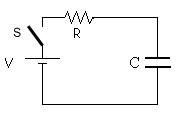
\includegraphics[width=6cm]{LG05--000.png}
    \caption{Esquema del circuito RC empleado.}
    \label{fig:circuitoRC}
\end{figure}

\subsection{Carga y descarga de un capacitor}

En esta primera etapa se estudia el proceso de carga y descarga del capacitor. 

\subsubsection{Midiendo en forma manual con mult\'\i metro}

De realizar la experiencia con cron\'ometro, se sugiere elegir valores de $R$ y
$C$ de manera tal que el producto $RC$ sea igual o superior a 100 segundos. De
esta forma los procesos de carga y descarga son lo sufientemente lentos como
para poder tomar los datos manualmente. 

\subsubsection{Midiendo a trav\'es de la placa de adquisici\'on SensorDAQ}

En cualquiera de las dos modalidades que se elija medir, se busca responder
las siguientes preguntas:
\begin{itemize}
    \item Cu\'al es el tiempo caracter\'\i stico (de carga y descarga) que se 
        obtiene de las  mediciones? Es el mismo para ambos procesos?
    \item Cu\'al es el valor de tensi\'on que se alcanza al llegar al 
        r\'egimen estacionario? 
    \item En el proceso de descarga, sobre que elemento disipativo se 
        descarga el capacitor?
    \item Es posible estimar la resistencia interna del mult\'\i metro? 
\end{itemize}

Repetir las mediciones utilizando otro valor de tensi\'on de trabajo $V'$
para la fuente. Observa cambios en el tiempo caracter\'\i stico producto de
esta modificaci\'on?

\section{Circuito RLC serie}

\subsection{Introducci\'on}

Considere el circuito RLC mostrado en la Figura \ref{fig:circuitoRLCserie}, en el
cual un capacitor $C$, una inductancia $L$ y una resistencia
$R$, se encuentran conectados en serie a un generador
de funciones $G$.

Aplicando las leyes de Kirchoff al circuito de la figura, 
tenemos:
\begin{equation}
    V_G = V_L + V_R + V_C = L \frac{dI}{dt} + RI + \frac{q}{C},
\end{equation}
ecuaci\'on que podemos derivar nuevamente para obtener
\begin{equation}
    \frac{dV}{dt} = L \frac{d^2I}{dt^2} + R \frac{dI}{dt} + \frac{I}{C}.
\end{equation}

Si el voltaje suministrado por el generador $G$ es sinusoidal, entonces el 
t\'ermino a la izquierda de la \'ultima ecuaci\'on es
\begin{equation}
    V(t) = V_m \sin \left( \omega t \right),
\end{equation}
y la corriente circulante por el circuito estar\'a dada por
\begin{equation}
    I(t) = I_m \sin \left( \omega t + \phi \right),
\end{equation}
siendo $\omega = 2\pi f$ la frecuencia angular, y $f$ la frecuencia 
(medida en Hz) suministrada por el generador de funciones. 

La impedancia $Z$ del circuito es 
\begin{equation}
    Z = Z_R + Z_L + Z_C = R + j \left( \omega L - \frac{1}{\omega C} \right),
\end{equation}
siendo $j$ la unidad imaginaria, por lo que
\begin{equation}
    V = IZ = I \left[ R + j \left( \omega L - \frac{1}{\omega C} \right) \right].
\end{equation}

Ahora bien, la tangente del \'angulo de desfasaje entre tensi\'on y corriente
ser\'a igual al cociente entre las partes imaginaria y real de la impedancia
$Z$, es decir:
\begin{equation}
    \tan \left( \phi \right) = \frac{\text{Im} Z}{\text{Re} Z} = 
    \frac{1}{R} \left(\omega L - \frac{1}{\omega C} \right),
\end{equation}
y el m\'odulo de la impedancia, resultar\'a
\begin{equation}
    |Z|^2 = R^2 + \left( \omega L - \frac{1}{\omega C} \right)^2.
\end{equation}

El \'angulo de desfasaje $\phi$ entre $I$ y $V$ puede ser positivo, en cuyo
caso el circuito es capacitivo. Si, por el contrario, $\phi < 0$, se dice que
el circuito es inductivo. Finalmente, si no hay desfasaje entre corriente y 
tensi\'on, el circuito se denomina resistivo. En este \'ultimo caso, tensi\'on
y corriente est\'an en fase y la parte imaginaria de la impedancia es nula.
Esta condici\'on implica
\begin{equation}
    \omega L - \frac{1}{\omega C} = 0,
\end{equation}
condici\'on que se cumple para la denominada {\it frecuencia de resonancia} 
$\omega_0$:
\begin{equation}
    \omega_0 = \frac{1}{\sqrt{LC}}.
\end{equation}
Resulta f\'acil observar que, para este caso, la corriente circulante por 
el circuito alcanza su amplitud m\'axima. En este marco, definimos el 
{\it ancho de banda} $\Delta \omega$ como el intervalo de frecuencias para
el que la potencia disipada disminuye exactamente a la mitad de la m\'axima
potencia disipada. De acuerdo a nuestros resultados anteriores, el 
ancho de banda para el circuito RLC serie viene dado por
\begin{equation}
    \Delta \omega = \frac{R}{L}.
\end{equation}
Definiendo ahora el {\it factor de calidad} o {\it m\'erito} $Q$ mediante
\begin{equation}
    Q = \frac{\omega_0}{\Delta \omega},
\end{equation}
obtenemos, para el caso del circuito que nos ocupa:
\begin{equation}
    Q = \frac{\omega_0 L}{R}.
\end{equation}

\subsection{Desarrollo de la experiencia}

En esta parte de la pr\'actica, se propone montar un circuito como el de la
Figura~\ref{fig:circuitoRLCserie}. A continuaci\'on:
\begin{enumerate}
    \item Estudie la variaci\'on de la tensi\'on sobre la resistencia en 
        funci\'on de la frecuencia de operaci\'on. 
    \item A partir de las mediciones realizadas en el inciso anterior,
        encuentre la frecuencia de resonancia y el valor del factor de
        calidad. Recuerde que la inductancia tiene una resistencia propia 
        (tal y como se muestra
        en la Figura~\ref{fig:circuitoRLCserie}) y, seg\'un corresponda,
        deber\'a ser considerada en la resistencia total del circuito.
    \item Determine experimentalmente el desfasaje $\phi(\omega)$ en funci\'on 
        de la frecuencia; para lo cual puede resultarle \'util el {\it modo XY}
        del osciloscopio. Para m\'as informaci\'on, consulte el apunte acerca
        de {\it C\'omo determinar el desfasaje entre dos se\~nales}.
\end{enumerate}

\begin{figure}[t!]
    \centering
    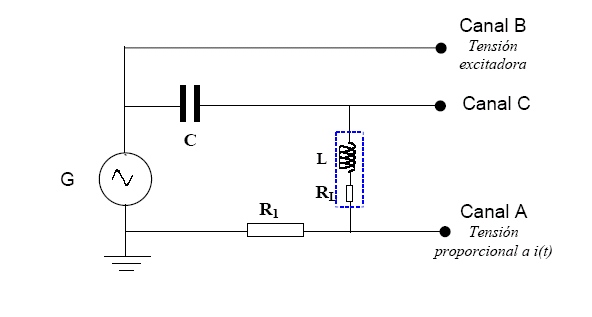
\includegraphics[width=9cm]{LG06--000.png}
    \caption{Esquema del circuito RLC serie.}
    \label{fig:circuitoRLCserie}
\end{figure}

\subsection{Desarrollo de la experiencia}

Para esta segunda parte de la pr\'actica, comience por montar el 
circuito de la
Figura~\ref{fig:circuitoRLCserie}. A continuaci\'on:
\begin{enumerate}
    \item Estudie la variaci\'on de la tensi\'on sobre la resistencia en 
        funci\'on de la frecuencia de operaci\'on. 
    \item A partir de las mediciones realizadas en el inciso anterior,
        encuentre la frecuencia de antiresonancia y el valor del factor de
        calidad.     
    \item Determine experimentalmente el desfasaje $\phi(\omega)$ en funci\'on 
        de la frecuencia; para lo cual puede resultarle \'util el {\it modo XY}
        del osciloscopio. Para m\'as informaci\'on, consulte el apunte acerca
        de {\it C\'omo determinar el desfasaje entre dos se\~nales}.
    \item Compare los resultados de esta parte con aquellos obtenidos en el
        estudio del circuito RLC serie.
\end{enumerate}

\begin{figure}[t!]
    \centering
    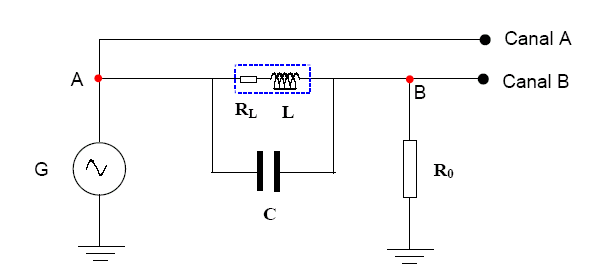
\includegraphics[width=9cm]{LG06--001.png}
    \caption{Esquema del circuito RLC paralelo.}
    \label{fig:circuitoRLCparalelo}
\end{figure}

\nocite{Alonso1998,Purcell1988,Reitz1996,Trelles1984,Reitz1996}
\bibliographystyle{unsrt} 
\bibliography{Bibliografia}

\end{document}
